\documentclass[ms,electronic,letterpaper,lol,lof,lot]{byumsphd}

% The following \documentclass options may be useful:
%
% 10pt          To set in 10-point type instead of 9-point.
% 11pt          To set in 11-point type instead of 9-point.
% authoryear    To obtain author/year citation style instead of numeric.

\usepackage{amsmath}
\usepackage{slatex}
\usepackage{graphicx}

\begin{document}

\title{Enabling Optimizations through Demodularization} 

\author{Blake Johnson}

\committeechair{Jay McCarthy}
\committeemembera{Eric Mercer}
\committeememberb{Quinn Snell}

\monthgraduated{March}
\yeargraduated{2013}
\yearcopyrighted{2013}


\documentabstract{%
Programmers want to write modular programs to increase maintainability and create abstractions, but modularity hampers optimizations, especially when modules are compiled separately or written in different languages. 
In languages with syntactic extension capabilities, each module in a program can be written in a separate language, and the module system must ensure that the modules interoperate correctly. 
In Racket, the module system ensures this by separating module code into phases for runtime and compile-time and allowing phased imports and exports inside modules. 
We present an algorithm, called demodularization, that combines all executable code from a phased modular program into a single module that can then be optimized as a whole program. 
The demodularized programs have the same behavior as their modular counterparts but are easier to optimize. 
We show that programs maintain their meaning through an operational semantics of the demodularization process and verify that performance increases by running the algorithm and existing optimizations on Racket programs.
}

\documentkeywords{macros, Racket, modules, optimization}

\acknowledgments{Acknowledged}

\department{Computer~Science}
\graduatecoordinator{Dan~Ventura}
\collegedean{Thomas~W.~Sederberg}
\collegedeantitle{Associate~Dean}
\maketitle


\chapter{Introduction}

Programmers should not have to sacrifice the software engineering goals of modular design and good abstractions for performance. 
Instead, their tools should make running a well-designed program as efficient as possible. 

Many languages provide features for creating modular programs which enable separate compilation and module reuse.
Some languages provide expressive macro systems, which enable programmers to extend the compiler in arbitrary ways.
Combining module systems with expressive macro systems allow programmers to write modular programs with each module written in its own domain-specific language.
A compiler for such a language must ensure that modular programs have the same meaning independent of the order in which the modules are compiled.
A phased module system, like the one described by Flatt \cite{Flatt} for Racket, is a way to allow both separately compiled modules and expressive macros in a language.

Modular programs are difficult to optimize because the compiler has little to no information about values that come from other modules when compiling a single module.
Existing optimizations have even less information when modules can extend the compiler. 
Good abstractions are meant to obscure internal implementations so that it is easier for programmers to reason about their programs, but this obscurity also limits information available for optimizations.  
In contrast, non-modular programs are simpler to optimize because the compiler has information about every value in the program.

Some languages avoid the problem of optimizing modular programs by not allowing modules, while others do optimizations at link time, and others use inlining. 
Not allowing modules defeats the benefits of modular design. 
Link time optimizations can be too low level to do useful optimizations. 
Inlining must be heuristic-based, and good heuristics are hard to develop. 

Our solution for optimizing modular programs, called demodularization, is to transform a modular program into a non-modular program by combining all runtime code and data in the program into a single module.
In a phased module system, finding all of the runtime values is not trivial.
Phased module systems allow programmers to refer to the same module while writing compiler extensions and while writing normal programs.
A demodularized program does not need to include modules that are only needed during compile-time, but whether or not the module is needed only at compile-time is not obvious from just examining the module in isolation. 

A program with a single module is effectively a non-modular program. After demodularization, a program becomes a single module, so existing optimizers have more information. Also, demodularization enables new optimizations that need whole program information. 

We provide an operational semantics for a simple language with a phased module system, and show that the demodularization process preserves program meaning. We also provide an implementation of demodularization for the Racket programming language, and verify experimentally that programs perform better after demodularization.

We explain demodularization at a high level with a detailed example (Chapter 2). Next, we use the operational semantics model of the demodularization process to explain why demodularization is correct (Chapter 3), then describe an actual implementation for Racket (Chapter 4), followed by experimental results of demodularizing and optimizing real-world Racket programs (Chapter 5). The operational semantics model removes the unnecessary details of the full implementation so the demodularization process is easier to understand and verify. The actual implementation presents interesting difficulties that the model does not. The experimental results show that demodularization improves performance, especially when a program is highly modular. 


\chapter{Intuition}

Demodularization enables whole-program optimizations and eliminates module loading overhead while maintaining the runtime meaning of a program.
To understand how demodularization preserves the runtime meaning of a program, we first need to understand the runtime meaning of a modular Racket program.
Consider the program in Figure~\ref{main-rkt}.

\begin{figure}[h]
\begin{schemedisplay}
#lang racket/base
(require "queue.rkt")

(with-queue (1 2 3 4 5 6)
  (enqueue 4)
  (displayln (dequeue))
  (displayln (dequeue)))
\end{schemedisplay}
\caption{\texttt{main.rkt}}
\label{main-rkt}
\end{figure}

This program imports a queue library through a \scheme{require} expression and then uses the library to do some queue operations.
Figures~\ref{queue-rkt}, \ref{long-queue-rkt}, and \ref{short-queue-rkt} contain the three modules that make up the queue library.
The library consists of a macro and two queue implementations, where the macro decides which implementation to use based on the length of the initial queue at compile time.

\begin{figure}[h]
\begin{schemedisplay}
#lang racket/base
(require (for-syntax racket/base
                     racket/syntax)
         "short-queue.rkt"
         "long-queue.rkt")

(define-syntax (with-queue stx)
  (syntax-case stx ()
    [(with-queue (v ...) e ...)
     (begin
       (define type 
         (if (> (length (syntax->list #'(v ...))) 5) 
	     'long 
             'short))
       (define make-queue 
         (format-id #'stx "make-~a-queue" type))
       (define enqueue (format-id #'stx "~a-enqueue" type))
       (define dequeue (format-id #'stx "~a-dequeue" type))
       #`(let ([q (#,make-queue v ...)])
           (define (#,(datum->syntax stx 'dequeue)) 
             (#,dequeue q))
           (define (#,(datum->syntax stx 'enqueue) x)
             (#,enqueue q x))
           e ...))]))

(provide with-queue)
\end{schemedisplay}
\caption{\texttt{queue.rkt}}
\label{queue-rkt}
\end{figure}

\begin{figure}[h]
\begin{schemedisplay}
#lang racket/base
(define (make-long-queue . vs)
  .... make-vector ....)

(define (long-enqueue q v)
  .... vector-set! ....)

(define (long-dequeue q)
  .... vector-ref ....)

(provide (all-defined-out))
\end{schemedisplay}
\caption{\texttt{long-queue.rkt}}
\label{long-queue-rkt}
\end{figure}

\begin{figure}[h]
\begin{schemedisplay}
#lang racket/base
(define (make-short-queue . vs)
  .... list ....)

(define (short-enqueue q v)
  .... cons ....)

(define (short-dequeue q)
  .... list-ref ....)

(provide (all-defined-out))
\end{schemedisplay}
\caption{\texttt{short-queue.rkt}}
\label{short-queue-rkt}
\end{figure}

The Racket runtime evaluates this program by compiling and then running the main module.
Whenever the runtime encounters a \scheme{require} expression during compilation, it either loads an existing compiled version of the required module or compiles the required module.
Whenever the runtime encounters a macro expression during compilation, it expands the macro.
In this example, the runtime begins to compile \texttt{main.rkt} and loads the compiled version of \scheme{racket/base}. 
Next, it encounters the \scheme{require} expression for \texttt{queue.rkt} and compiles it.
Compilation of \texttt{queue.rkt} triggers compilation of both \texttt{short-queue.rkt} and \texttt{long-queue.rkt}. 

After finishing \texttt{queue.rkt}, the runtime returns to \texttt{main.rkt} and expands the \scheme{with-queue} macro.
The \scheme{with-queue} macro checks the length of the initial queue, which in this case is six, and chooses to use the \scheme{long-queue} implementation.
The macro expands into a \scheme{let} expression that binds the identifier \scheme{q} to the initial queue, along with internal definitions of \scheme{enqueue} and \scheme{dequeue} that use the \scheme{long-queue} implementations.
Figure~\ref{main-expanded-rkt} shows what \texttt{main.rkt} looks like after expansion.

\begin{figure}[h]
\begin{schemedisplay}
(module main racket/base
  (#%module-begin
   (require "queue.rkt")
   (let ((q (make-long-queue 1 2 3 4 5 6)))
     (define (dequeue) (long-dequeue q))
     (define (enqueue x) (long-enqueue q x))
     (enqueue 4)
     (displayln (dequeue))
     (displayln (dequeue)))))
\end{schemedisplay}
\caption{\texttt{main.rkt} expanded}
\label{main-expanded-rkt}
\end{figure}


After compiling the whole program, the Racket runtime evaluates the program by loading and executing the compiled main module.
As is the case with compilation, evaluation also follows the \scheme{require} expressions and runs required modules as it encounters them.
In this example, the runtime evaluates \texttt{main.rkt} and encounters the \scheme{require} expression for \texttt{queue.rkt}.
It then follows the \scheme{require}s for \texttt{short-queue.rkt} and \texttt{long-queue.rkt} and installs the definitions that those modules provide.
When evaluation returns to \texttt{queue.rkt}, nothing else happens because macros are only needed at compile time.
Finally, evaluation returns to \texttt{main.rkt} and the runtime evaluates the rest of the program.

A demodularized version of this program should contain all code that ran while evaluating the modular program, minus the module loading steps.
The demodularization algorithm starts with the compiled versions of all of the modules for the program, and then traces the \scheme{require} expressions and includes all runtime code into a single module in the order it encounters the code.
Figure~\ref{main-demod-rkt} shows what the single module looks like after running the demodularization algorithm on it.
There are no require statements and the macro definition is gone, but the all the code that ran during the evaluation of the modular version is there in the same order as before.

\begin{figure}[h]
\begin{schemedisplay}
(module main racket/base
  (#%module-begin
   (define (make-short-queue . vs)
    .... list ....)

   (define (short-enqueue q v)
    .... cons ....)

   (define (short-dequeue q)
    .... list-ref ....)

   (define (make-long-queue . vs)
    .... make-vector ....)

   (define (long-enqueue q v)
    .... vector-set! ....)

   (define (long-dequeue q)
    .... vector-ref ....)

   (let ((q (make-long-queue 1 2 3 4 5 6)))
     (define (dequeue) (long-dequeue q))
     (define (enqueue x) (long-enqueue q x))
     (enqueue 4)
     (displayln (dequeue))
     (displayln (dequeue)))))
\end{schemedisplay}
\caption{\texttt{main.rkt} demodularized}
\label{main-demod-rkt}
\end{figure}


This example is rather simple because it only uses a single macro, but in practice, Racket programs use many macros, even macros that use other macros in their implementations, creating a language tower.
The demodularization algorithm takes this into account by only gathering runtime code while tracing through \scheme{require} expressions.
The details about how this works is further explained in the operational semantics model in Chapter 3.

With all of the code in a single module, it is easy to see how standard optimizations such as inlining and dead code elminiation can reduce the module to the code in Figure~\ref{main-demod-opt-rkt}.
\begin{figure}[h]
\begin{schemedisplay}
(module main racket/base
  (#%module-begin
   (let ((q (.... make-vector .... 1 2 3 4 5 6 ....)))
     (.... vector-set .... 4 ....)
     (displayln (.... vector-ref ....))
     (displayln (.... vector-ref ....)))))
\end{schemedisplay}
\caption{\texttt{main.rkt} demodularized and optimized}
\label{main-demod-opt-rkt}
\end{figure}
In this simple example, with constant folding this progam could be optimized even more, but even in programs with dynamic inputs, demodularization enables many optimizations that aren't possible when the program is separated into modules.

\chapter{Model}

We can understand the specifics of demodularization by describing it as an algorithm for a simple language with a well defined semantics.
The \emph{mod} language (Figure~\ref{source-lang}) contains only the features necessary to write modular programs where it is possible to observe the effects of module evaluation order.

\begin{figure}[h]
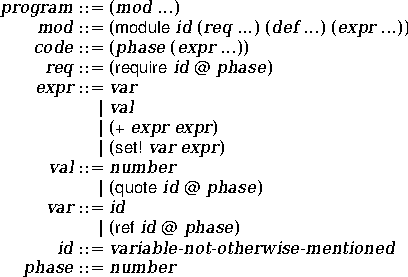
\includegraphics{source}
\caption{\emph{mod} language grammar}
\label{source-lang}
\end{figure}

A program in \emph{mod} consists of a list of modules that can refer to each other.
Each module has a name, any number of imports, any number of definitions, and sequenced code expressions. 
All definitions in a module are exposed as exports to other modules, but to use definitions from another module, the program must import it through a \scheme{require} expression.
Both \scheme{require} and \scheme{define} expressions have phase annotations; this simulates the interactions between modules in a language with macros and a language tower without requiring a model of macro expansion.
The language includes variable references, numbers, addition, and mutation.
Mutation makes module evaluation order observable, and addition represents the work that a module does.
In addition to numbers and variables, there are two special forms of values and references that model the interaction of macros with the module system.
A \scheme{quote} expression is like a reference to syntax at runtime.
A \scheme{ref} expression is like a macro that can only do one thing: refer to a variable at a phase.

The \emph{mod} language exposes phases as an integral part of the language, while languages like Racket keep phases obscured from the end user even though it uses phases during compiling and evaluating a program.
So, what is a phase?
In the discussion of the example program in section XXX, we used the terminology of runtime and compile-time.
Phases are just numerical designations for these terms, where runtime is phase 0 and compile-time is phase 1.
The reason phases are numbers is because phases exist outside of the range of 0 to 1.
Given that phase 1 is the compile-time for phase 0, we can extend this idea so that phase 2 is the compile-time for phase 1.
Conversely, compile-time code generates code for the phase below it, so it can refer to bindings at negative phases.
(Talk about relative phases)
Phases allow programmers to build syntactic abstractions that use other syntactic abstractions, creating a tower of intermediate languages.
The \emph{mod} language does not allow programmers to create language towers, but evaluating a \emph{mod} program uses the same mechanisms as evaluating a Racket program.

We have to compile \emph{mod} programs before demodularizing them, just like in the Racket implementation.
In Racket, compiling expands all macros in a program and changes definitions and variable references to refer to memory locations.
In \emph{mod}, compiling eliminates \scheme{ref} expressions, turns definitions into \scheme{set!} expressions, changes variable references to include module information, and sorts code into phases.
Compilation in both cases still leaves behind a relatively high-level language, but the language is free of syntactic extensions.
This is important for demodularization because otherwise macro expansion would have to be part of the algorithm, which would complicate it and possibly duplicate work.
The grammar in Figure~\ref{compiled-lang} specifies the compiled language for \emph{mod}.

\begin{figure}[h]
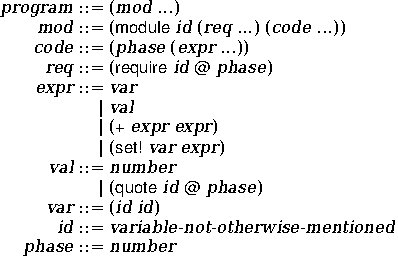
\includegraphics{compiled-lang}
\caption{compiled language grammar}
\label{compiled-lang}
\end{figure}

We evaluate the compiled language using a small-step reduction semantics. 
Because the reduction rules are syntactic, we extend the compiled language further with evaluation contexts, a heap representation, and a stack representation to keep track of the order to instantiate modules.
These extensions are in Figure~\ref{compiled-eval-lang}.
An expression of the form:
\setspecialsymbol{sigma}{$\sigma$}
\begin{schemedisplay}
(sigma / (mod ...) / ((id phase) ...)  / ((id phase) ...))
\end{schemedisplay}
represents the state of the machine during evaluation.
$\sigma$ represents the heap of the program, and when evaluation finishes represents the output of the program.
The list of modules is the code of program in the compiled language.
The first list of \scheme{(id phase)} pairs is the list of modules to evaluate, and the second list is the modules that have already been evaluated.

\begin{figure}[h]
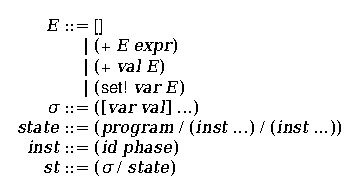
\includegraphics{compiled-eval-lang}
\caption{extensions to compiled language grammar}
\label{compiled-eval-lang}
\end{figure}

The reduction rules in Figure~\ref{eval-reduction} evaluate a compiled program that starts with an empty heap, the program code, a stack that contains the identifier of the main module at phase 0, and an empty completed module list. 

\begin{figure}[h]
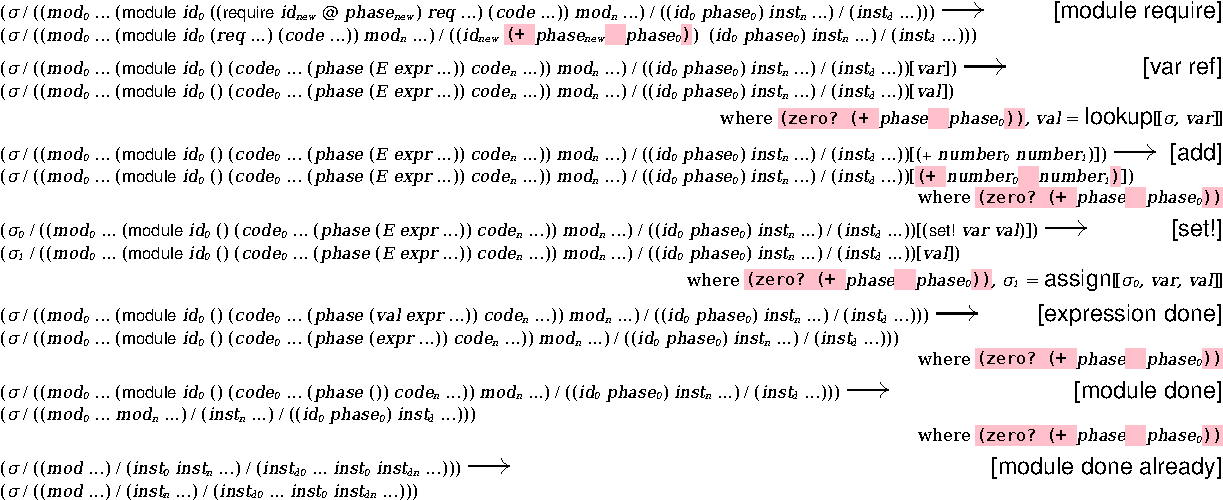
\includegraphics[width=\textwidth]{eval-reduction}
\caption{modular evaluation}
\label{eval-reduction}
\end{figure}

The \emph{module require} rule matches a program with a \scheme{require} expression in the module at the top of the evaluation stack and evaluates it by removing the \scheme{require} expression from the module and pushing the required module onto the evaluation stack with the phase shifted appropriately.
The current module is still on the stack and will continue evaluating after the required module is done evaluating.
The subsequent rules all apply only when the phase relative to the main module is zero.
The \emph{var ref} rule looks up a variable in the heap and replaces the variable with its current value.
The \emph{add} rule replaces an addition expression of numbers with the result of computing their sum.
The \emph{set!} rule installs a value for a variable into the heap and reduces to the value.
When an expression is a value, the \emph{expression done} rule matches and removes the expression from the module.
When there are no more expressions left in a module, the \emph{module done} rule applies by removing the module from the program and placing a reference to it in the list of finished modules.
The \emph{module done already} rule applies when the current module on the stack is in the finished list, so that modules are not evaluated multiple times. 

Figure~\ref{demod-redex} shows the demodularization algorithm for the compiled language.
\begin{figure}[h]
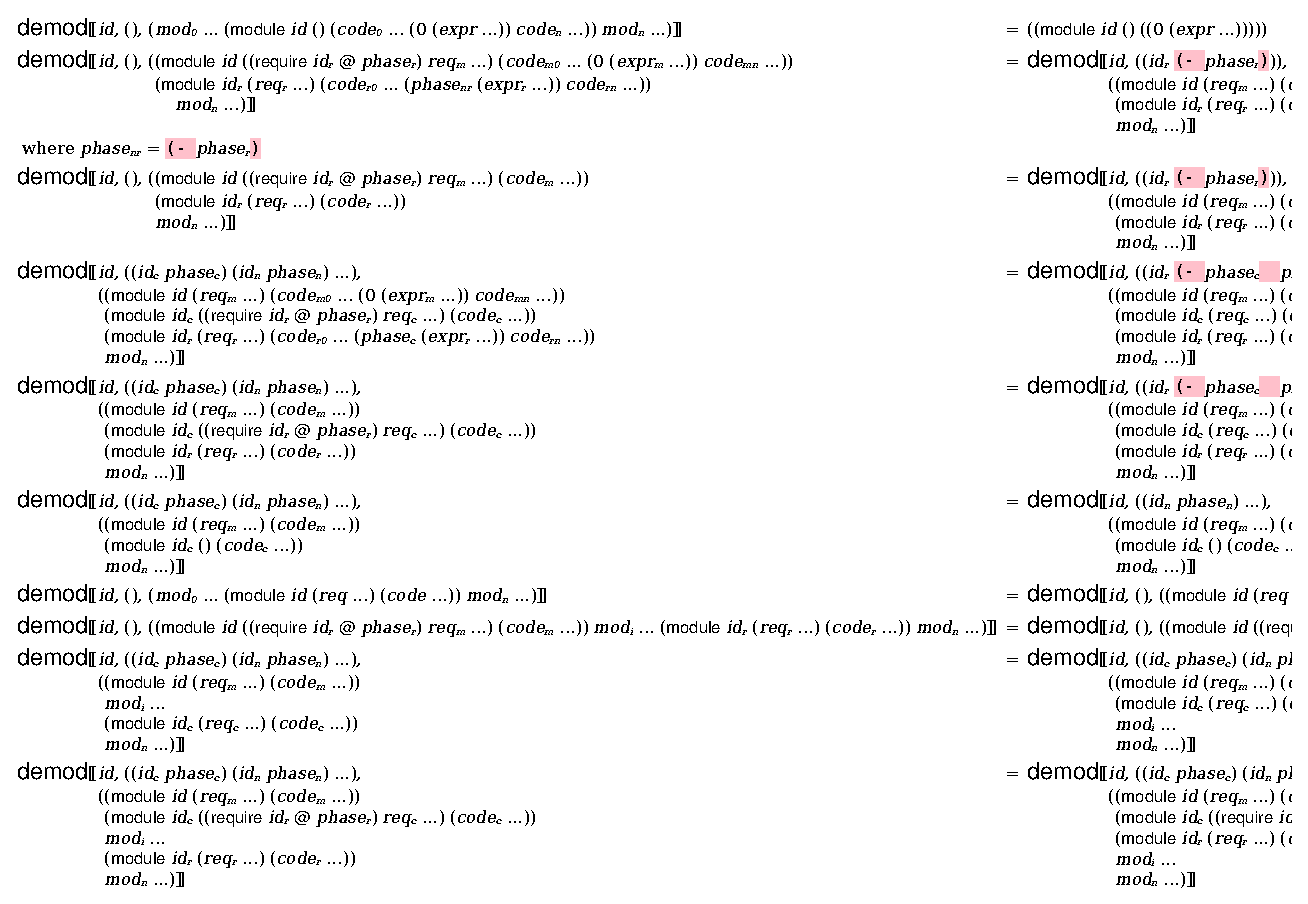
\includegraphics[width=\textwidth]{demod-redex}
\caption{Demodularization algorithm}
\label{demod-redex}
\end{figure}

\chapter{Implementation}

The demodularization algorithm for the Racket module system operates on Racket bytecode. 
Racket's bytecode format is one step removed from the fully-expanded kernel language: instead of identifiers for bindings, it uses locations.
For toplevel bindings, these locations point to memory allocated for each module known as the module's prefix.
So, in \texttt{long-queue.rkt}, \scheme{make-long-queue} would be in prefix location 0 and \scheme{long-enqueue} would be in prefix location 1, and all the references to \scheme{make-long-queue} and \scheme{long-enqueue} are replaced with references to 0 and 1.
Like in the model, the algorithm combines all phase 0 code into a single module, but since the references are locations instead of identifiers, the locations of different modules overlap.
We solve this by extending the prefix of the main module to have locations for the required module's toplevel identifiers, and then adjusting the toplevel references in the required module to those new locations. 

After combining all the code for a program into a single module, we want to optimize it.
The existing optimizations for Racket operate on an intermediate form that is part way between fully-expanded code and bytecode. 
Therefore, to hook into the existing optimizations, we decompile the bytecode of the demodularized program into the intermediate form and then run it through the optimizer to produce bytecode once more.

Racket provides features that treat modules as first-class objects during runtime. 
For example, programs can load and evaluate modules at runtime through \scheme{dynamic-require}. 
These features can work with demodularization, but the onus is on the programmer to make sure to use the features in particular ways.
The main restriction is that the program cannot share a module that is part of the demodularized program and also part of a dynamically required module. 
This restriction may seem easy to follow in theory, but in practice it is hard because most modules rely on built-in Racket libraries that will be in both the static and dynamic parts of the program.

\chapter{Evaluation}

We tested our implementation of demodularization by selecting existing Racket programs and measuring their execution time before and after demodularization.
We also measured the memory usage and compiled bytecode size of the programs.
We ran the benchmarks on an Intel Core 2 Quad machine running Ubuntu and ran each program X times.
We expect programs to perform better based on how modular the program is, which we measure by counting the number of modules in a program's require graph and how many cross module references occur in the program.

Figure XXX shows the results of running this experiment on XXX Racket programs. 
On one end of the spectrum, there are programs like XXX which are already basically single module programs, so demodularization does little besides rerun the optimizer on the program. Running the optimizer again may have positive or negative effects on performance, it may unroll loops and inline definitions more aggressively the second time, but some of these ``optimizations" may hurt performance.
On the other end of the spectrum, highly modular programs like XXX perform much better after demodularization.
We expect performance to increase at a linear or even superlinear pace as modularity increases because of the extra information available to the optimizer.

This experiment uses only the existing Racket optimizations, which are intra-module optimizations.
Certain optimizations that are not worthwhile to do at the intra-module level have larger payoffs when applied to whole programs. 
With demodularization, we anticipate that new whole-program optimizations enabled by demodularization will increase performance even more.

\chapter{Related Work}
Prior work on whole-program optimization has come in two flavors, depending on how much access to the source code the optimizer has. The first approach assumes full access to the source code and is based on inlining. The second approach only has access to compiled modules and is based on combining modules.

The first approach is based on selectively inlining code across module boundaries because it has full access to the source code of the program \cite{258960,Chambers96whole-programoptimization}. Most of the focus of this approach is finding appropriate heuristics to inline certain functions without ballooning the size of the program and making sure the program still produces the same results. Resulting programs are not completely demodularized; they still have some calls to other modules. Specifically, Chambers et al. \cite{Chambers96whole-programoptimization} show how this approach applies to object-oriented languages like C++ and Java, where they are able to exploit properties of the class systems to choose what to inline. Blume and Appel \cite{258960} showed how to deal with inlining in the presence of higher order functions, to make sure the semantics of the program didn't change due to inlining. Their approach led to performance increases of around 8\%.

The second approach is taking already compiled modules, combining them into a single module, and optimizing the single module at link time \cite{sutter,727617}. Most of the work done with this approach optimized at the assembly code level, but because they were able to view the whole program, the performance increases were still valuable. 
The link-time optimization system by Sutter et al. \cite{sutter} achieves a 19\% speedup on C programs.
One of the reasons for starting with compiled modules is so that programs using multiple languages can be optimized in a common language, like the work done by Debray et al. \cite{727617} to combine a program written in both Scheme and Fortran. The main problem with this approach is that the common language has less information for optimization than the source code had. 
These approaches are similar to demodularization, but the operate at a lower level and work on languages without phased module systems.

\chapter{Conclusion}

Demodularization is a useful optimization for deploying modular programs. 
A programmer can write a modular program and get the benefits of separate compilation while devloping the program, and then get additional speedups by running the demodularizer on the completed program.
Demodularization also enables new optimizations that are not feasible to implement for modular programs.
Without module boundaries, inter-procedural analysis is much easier and worthwhile.
Also, dead code elmination works much better because the whole program is visible, while in a modular program, only dead code that is private to the module can be eliminated.

In the future, we would like to implement an aggressive dead code elimination algorithm for Racket.
We implemented a naive one that does not respect side effects, but shows the potential gains from this optimization; it is able to shrink Racket binaries down from about 2MB to about 100KB.
This promising result implies that other low-hanging optimizations should be possible on demodularized programs that can increase performance.

\bibliographystyle{plain}
\bibliography{bib}

\end{document}
